\documentclass[a4paper,9pt]{report}

\usepackage{subfig}
\usepackage{float}
\usepackage[myheadings]{fullpage}
\usepackage{fancyhdr}
% \usepackage[T1]{fontenc}
\usepackage[english]{babel}
\usepackage{amsmath}
\usepackage{bbold}

\newcommand{\HRule}[1]{\rule{\linewidth}{#1}}

\pagestyle{fancy}
\fancyhf{}
\setlength\headheight{15pt}
\fancyhead[R]{Introduction to Natural Language Processing}

\usepackage[english]{babel}
\usepackage[letterpaper,top=2cm,bottom=2cm,left=3cm,right=3cm,marginparwidth=1.75cm]{geometry}

\usepackage{amsmath}
\usepackage{graphicx}
\usepackage[colorlinks=true, allcolors=blue]{hyperref}

\begin{document}

\title{ \normalsize \textsc{\LARGE Neural Pos Tagging}
		\\ [2.0cm]
		\HRule{0.5pt} \\
		\LARGE \textbf{\uppercase{Report}}
		\HRule{2pt} \\ [0.5cm]
		\normalsize \vspace*{3\baselineskip}}
        \date{ }

\author{Ashmit Chamoli }

\maketitle
\section*{Introduction}
This report contains training and testing details for neural PoS tagging architectures presented in this repository.

Two architectures are used in this report, based on ANN and LSTM respectively. The implementation details of both these architectures can be found in the README.

\section*{Dataset}
For training, the \href{https://lindat.mff.cuni.cz/repository/xmlui/bitstream/handle/11234/1-5287/ud-treebanks-v2.13.tgz}{Univeral Dependencies} dataset has been used. Specifically, the file located in the \verb|UD_English-Atis/| folder are used.
For parsing this dataset,the \href{https://pypi.org/project/conllu/}{conllu} library has been used. 

\section*{Training}
\subsection*{ANN PoS Tagger}
To tune the hyperparameters for this model, a grid search was performed on the following sets of hyperparameters:
\begin{itemize}
    \item Embedding Sizes: 128, 256, 512
    \item Hidden Layers: [], [32], [64], [128], [128, 64], [64, 32]
    \item Activation: RelU, Sigmoid, Tanh
    \item Context Sizes: 0, 1, 2, 3, 4  
\end{itemize}
All models were trained for 15 epochs with a batch size of 128 and a learning rate of 0.001. Evaluation metrics (accuracy, precision, recall and f1-score) were evaluated on the train set, dev set and the test set for each of the 270 models trained.

The following were the top 5 models based on dev set f1-score:
\begin{table}[H]
    \centering
    \begin{tabular}{|c|c|c|c|c|c|}
        \hline
        \textbf{Rank} & \textbf{Embedding Size} & \textbf{Hidden Layer} & \textbf{Activation} & \textbf{Context Size} & \textbf{Dev F1} \\
        \hline
        1 & 512 & [64, 32] & 'tanh' & 3 & 0.982 \\
        \hline                                            
        2  & 256 & [128] & 'sigmoid' & 2 & 0.982 \\
        \hline
        3 & 128 & [128] & 'relu' & 2 & 0.982 \\
        \hline
        4 & 256 & [128] & 'tanh' & 1 & 0.982 \\
        \hline        
        5 & 128 & [] & 'tanh' & 1 & 0.982 \\
        \hline
    \end{tabular}
\end{table}

The following is the plot of training progress of the best ANN model:
\begin{figure}[H]
    \centering
    \resizebox{\textwidth}{!}{
        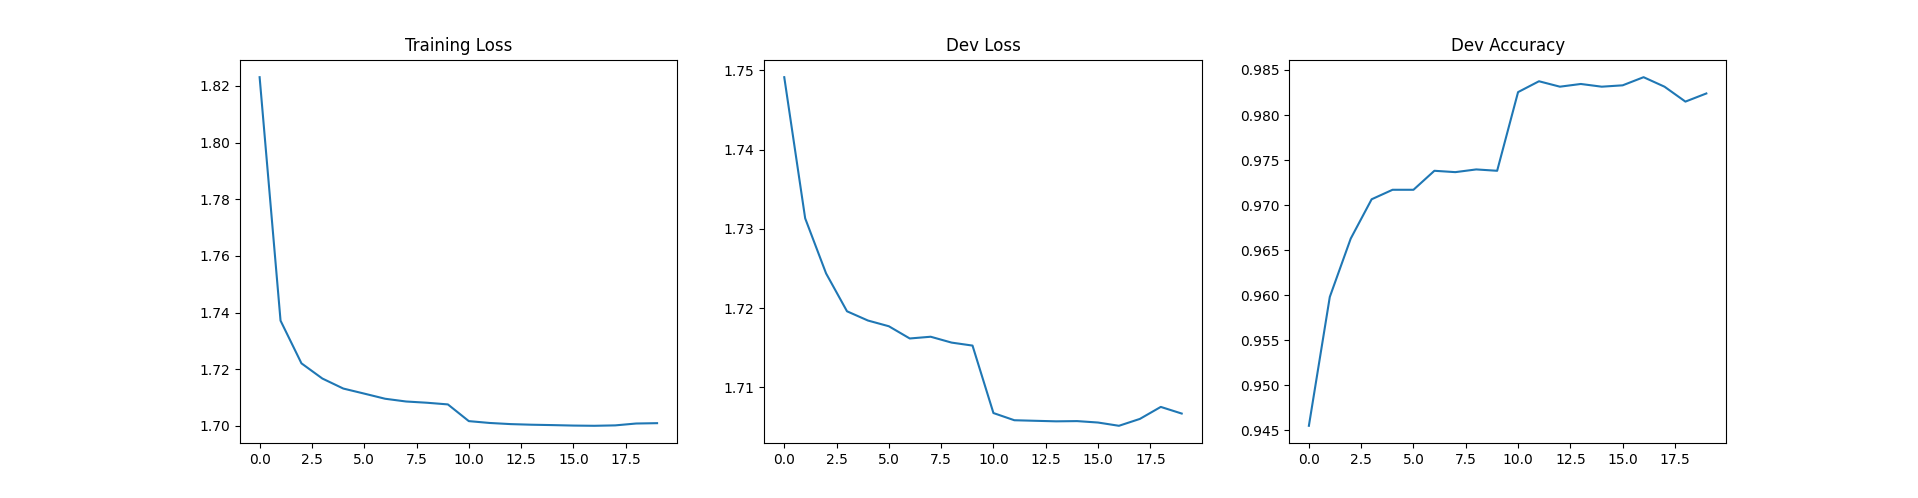
\includegraphics[scale=0.4]{../plots/annTrainingProgress.png}
    }
    \caption*{The plot shows various training metrics accross epochs. As expected all the metrics improve after each epoch.}
\end{figure}
This graph is expected. 
We will now look at the confusion matrix for the best model.
\begin{figure}[H]
    \centering
    \resizebox{\textwidth}{!}{
        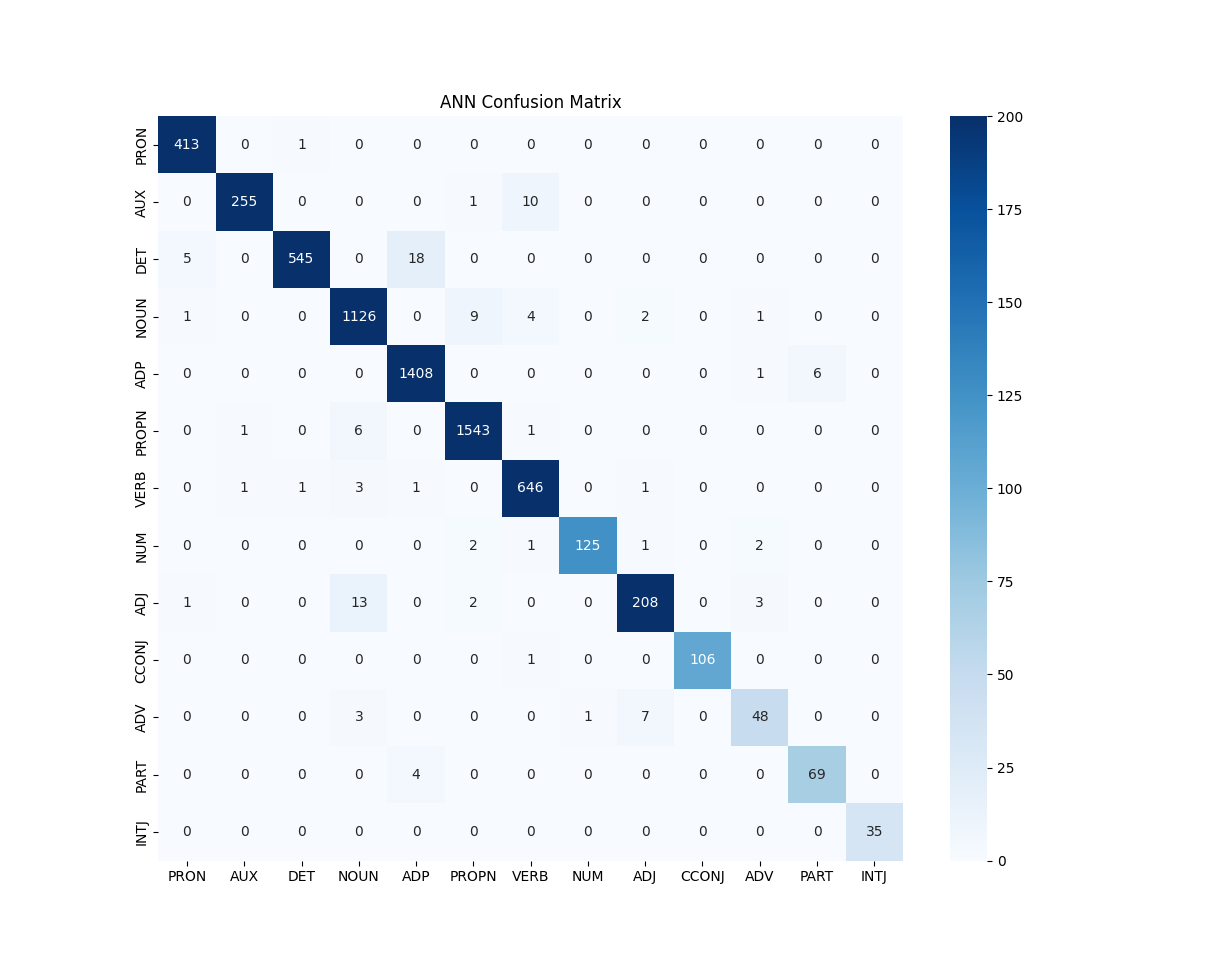
\includegraphics[scale=0.4]{../plots/annConfusionMatrix.png}
    }
    \caption*{The confusion matrix for the best ANN model.}
\end{figure}
As is evident by the confusion matrix, the model is performing really well for most classes. However the model is slightly confused between adverbs and adjectives and predicting 22\% of the adverbs as adjectives. This is an interesting observation because adverbs and adjectives are often difficult to tell apart even for humans. Another interesting observation is that the model almost never confuses adjectives for adverbs, that is, it almost always classifies adjectives correctly.

Next, we will plot accuracy vs context size for the best model.

\begin{figure}[H]
    \centering
    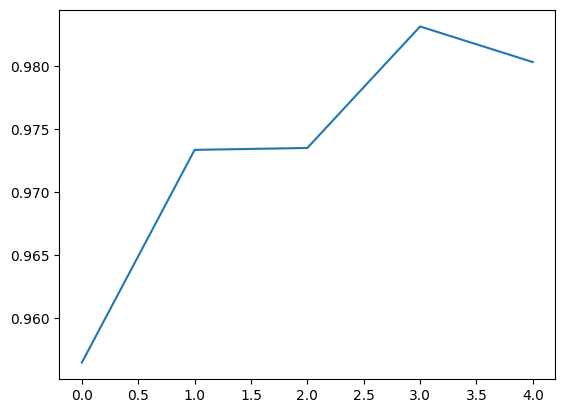
\includegraphics[scale=0.4]{../plots/accuracyVsContextSize.png}    
    \caption*{The plot shows accuracy vs context size for the best ANN model.}
\end{figure}

We can see that the accuracy is highest when context size is 3. A context size of 4 is too much and is probably adding noise to the data points. On the other hand a context size of lower than 3 provides less amount of information and thus the model performance decreases.

\subsection*{RNN PoS Tagger}
To tune the hyperparameters for this model, a grid search was performed on the following sets of hyperparameters:
\begin{itemize}
    \item Embedding Size: 128, 256
    \item Hidden Embedding Size: 64, 128
    \item Hidden Layers: [64], [32, 16], [64, 32]
    \item Number of Stacks: 1, 2, 3
\end{itemize}
For all the models, learning rate, epochs and activation was set to 0.001, 13 and RelU respectively.

The top 5 models based on dev set f1-score are:

\begin{table}[H]
    \centering
    \begin{tabular}{|c|c|c|c|c|c|c|}
        \textbf{Rank} & \textbf{Embedding Size} & \textbf{Hidden Embedding Size} & \textbf{Hidden Layers} & \textbf{Number of Stacks} & \textbf{Dev F1} \\
        \hline
        1 & [64, 32] & 256 & 64 & 2 & 'relu' & 0.971081 \\
        \hline
        2 & [64, 32] & 256 & 128 & 2 & 'relu' & 0.971079 \\
        \hline
        3 & [64] & 128 & 128 & 2 & 'relu' & 0.971017 \\
        \hline
        4 & [32, 16] & 256 & 128 & 2 & 'relu' & 0.970926 \\
        \hline
        5 & [32, 16] & 256 & 128 & 3 & 'relu' & 0.97083 \\

    \end{tabular}
\end{table}

\section*{Perplexity Scores}
For each of the 2 corpora provided, we construct a test set by selecting 1000 sentences at random and a train set containing the rest of the sentences. We calculate the perplexity of each sentence and report the average over all sentences for each language model.

\subsection*{LM 1: Tokenization + 3-gram LM + Good-Turing Smoothing}
\subsubsection*{Pride and Prejudice}
\begin{table}[H]
    \centering
    \begin{tabular}{|c|c|}
        \hline
        \textbf{Train} & {90651.12} \\
        \hline
        \textbf{Test} & {12722.59} \\
        \hline
    \end{tabular}
\end{table}
The high perplexity values on the test set indicate that the model is quite confused about it's prediction. The higher value of perplexity in the train set is because Good Turing smoothing assigns a very high probability to unseen n-grams which in turns results in probability of seen but low frequency n-grams to be extremely low. 
In the test set however, we see a lot of unseen n-grams for which the good turing model returns a very high probability.

\subsubsection*{Ulyess}
\begin{table}[H]
    \centering
    \begin{tabular}{|c|c|}
        \hline
        \textbf{Train} & {215313.48} \\
        \hline
        \textbf{Test} & {16327.17} \\
        \hline
    \end{tabular}
\end{table}
Here similar trend is followed, except that the train perplexity is much higher than we see in Pride and Prejudice. This is because of a much larger vocabulary set and a larger dataset. This results in the probability of unseen n-grams to be even higher than was the case in Pride and Prejudice dataset.

\subsection*{LM 2: Tokenization + 3-gram LM + Linear Interpolation}
\subsubsection*{Pride and Prejudice}
\begin{table}[H]
    \centering
    \begin{tabular}{|c|c|}
        \hline
        \textbf{Train} & {27.70} \\
        \hline
        \textbf{Test} & {813.61} \\
        \hline
    \end{tabular}
\end{table}


\subsubsection*{Ulyess}
\begin{table}[H]
    \centering
    \begin{tabular}{|c|c|}
        \hline
        \textbf{Train} & {97.05} \\
        \hline
        \textbf{Test} & {2463.43} \\
        \hline
    \end{tabular}
\end{table}

The perplexity in the for the train sets is quite low, indicating that the model is quite sure of it's prediction. 
On the test sets however, the overall perplexity is much lower than we see in Good Turing, meaning that the model is performing better in this case.

The perplexity scores are always higher for the Ulyess dataset as compared to the Pride and Prejudice dataset. This might be because of the richer vocabulary in the Ulyess dataset.

The best performance we achieve is by LM2 on the Pride and Prejudice dataset.

\end{document}
